% This must be in the first 5 lines to tell arXiv to use pdfLaTeX, which is strongly recommended.
\pdfoutput=1
% In particular, the hyperref package requires pdfLaTeX in order to break URLs across lines.

\documentclass{article}

% if you need to pass options to natbib, use, e.g.:
%     \PassOptionsToPackage{numbers, compress}{natbib}
% before loading neurips_2026

% The authors should use one of these tracks.
% Before accepting by the NeurIPS conference, select one of the options below.
% 0. "default" for submission
% \usepackage{neurips_2026}
% the "default" option is equal to the "main" option, which is used for the Main Track with double-blind reviewing.
% 1. "main" option is used for the Main Track
% \usepackage[main]{neurips_2026}
% 2. "position" option is used for the Position Paper Track
%  \usepackage[position]{neurips_2026}
% 3. "eandd" option is used for the Evaluations & Datasets Track
% \usepackage[eandd]{neurips_2026}
% if you want to opt-in for a de-anomymized submission (not recommended, but OK):
%\usepackage[eandd, nonanonymous]{neurips_2026}
% 4. "creativeai" option is used for the Creative AI Track
%  \usepackage[creativeai]{neurips_2026}
% 5. "sglblindworkshop" option is used for the Workshop with single-blind reviewing
% \usepackage[sglblindworkshop]{neurips_2026}
% 6. "dblblindworkshop" option is used for the Workshop with double-blind reviewing
%  \usepackage[dblblindworkshop]{neurips_2026}

% After being accepted, the authors should add "final" behind the track to compile a camera-ready version.
% 1. Main Track
\usepackage[main, preprint]{neurips_2026}
% 2. Position Paper Track
%  \usepackage[position, final]{neurips_2026}
% 3. Evaluations & Datasets Track
% \usepackage[eandd, final]{neurips_2026}
% 4. Creative AI Track
%  \usepackage[creativeai, final]{neurips_2026}
% 5. Workshop with single-blind reviewing
%  \usepackage[sglblindworkshop, final]{neurips_2026}
% 6. Workshop with double-blind reviewing
%  \usepackage[dblblindworkshop, final]{neurips_2026}
% Note. For the workshop paper template, both \title{} and \workshoptitle{} are required, with the former indicating the paper title shown in the title and the latter indicating the workshop title displayed in the footnote.
% For workshops (5., 6.), the authors should add the name of the workshop, "\workshoptitle" command is used to set the workshop title.
% \workshoptitle{WORKSHOP TITLE}

% "preprint" option is used for arXiv or other preprint submissions
% \usepackage[preprint]{neurips_2026}

% to avoid loading the natbib package, add option nonatbib:
%    \usepackage[nonatbib]{neurips_2026}

\usepackage[utf8]{inputenc} % allow utf-8 input
\usepackage[T1]{fontenc}    % use 8-bit T1 fonts
\usepackage{hyperref}       % hyperlinks
\usepackage{url}            % simple URL typesetting
\usepackage{booktabs}       % professional-quality tables
\usepackage{amsmath}        % math environments and \text
\usepackage{amsfonts}       % blackboard math symbols
\usepackage{nicefrac}       % compact symbols for 1/2, etc.
\usepackage{microtype}      % microtypography
\usepackage{xcolor}         % colors
\usepackage{tabularx}
\usepackage{caption}
\usepackage{subcaption}
\usepackage{orcidlink}
\usepackage{algorithm}
\usepackage{algpseudocode}

\begin{document}

\title{Language steering in latent space to mitigate unintended code-switching}

\author{
  Andrey Goncharov\orcidlink{0009-0006-9471-2181}\\
  Applied AI Institute\\
  \texttt{andrey@faillearnrepeat.net}
  \And
  Nikolai Kondusov\\
  Voronezh State University
  \And
  Alexey Zaytsev\orcidlink{0000-0002-1653-0204}\\
  Applied AI Institute
}

\maketitle

\begin{abstract}
  Multilingual Large Language Models (LLMs) often exhibit hallucinations such as unintended code-switching, reducing reliability in downstream tasks.
  We propose latent-space language steering, a lightweight inference-time method that identifies a language direction via Principal Component Analysis (PCA) on parallel translations
  and steers embeddings along this axis to control language identity.
Our approach reduces next-token distributional divergence by up to 55\%, Code-Switching Index by 63--99\%, while preserving broad semantic direction with negligible computational overhead
and requires only minimal parallel data for calibration.
\end{abstract}

% \keywords{large language models \and multilingual \and code-switching \and representation engineering \and activation steering \and latent space \and principal component analysis}

\section{Introduction}

\begin{figure}[ht]
  \centering
  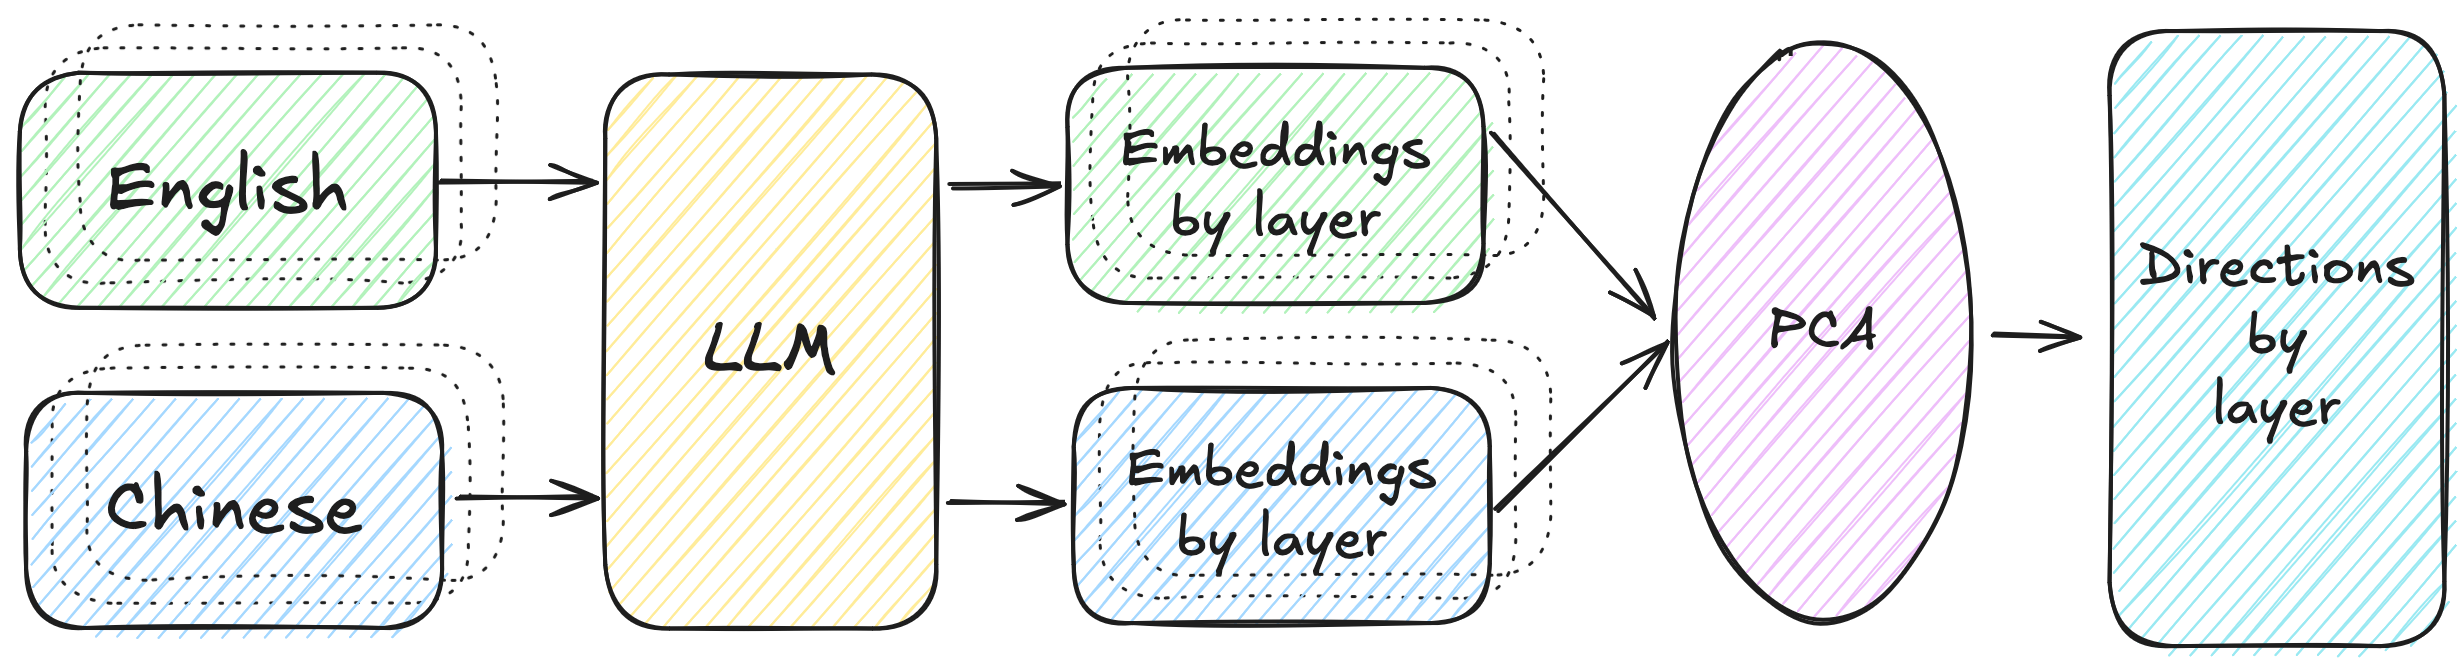
\includegraphics[width=1\linewidth]{images/language_steering_scheme.png}
  \caption{Language steering in hidden space: 1. Collect parallel translations of the same concepts; 2. LLM forward pass to get embeddings by layer; 3. Perform PCA by layer on the merged embeddings.}
  \label{fig:lang_steering_scheme}
\end{figure}

LLMs exhibit unintended code-switching - generating tokens in languages other than the target~\citep{marchisio-etal-2024-understanding}.
\citet{ryan-etal-2024-unintended} document how LLM alignment procedures can cause models to default to English even when prompted in other languages,
\citet{yoo2025codeswitchingredteamingllmevaluation} demonstrate that code-switching serves as an effective red-teaming vector, bypassing safety filters.
Existing solutions require costly fine-tuning~\citep{marchisio-etal-2024-understanding} or introduce latency via decoding-time interventions~\citep{dathathri2020plugplaylanguagemodels, yang-klein-2021-fudge, liu2021dexpertsdecodingtimecontrolledtext}.

We propose \emph{latent space language steering}, a cheap inference-time method that exploits low-dimensional language directions in hidden representations.
By applying PCA to parallel translations, we identify linear subspaces separating languages while preserving broad semantic direction.
Steering via simple projection (one dot product and vector subtraction per token) mitigates code-switching with negligible overhead.

Additionally, we analyze language clustering dynamics across layers and discover that a single final layer projection enables near-perfect language classification. Code and data are released to facilitate further research \footnote{\url{https://github.com/fxlrnrpt/language-steering-in-latent-space}}.


\section{Related works}

\label{sec:related}

\paragraph{Code-switching and multilingual control.}
While code-switching has been studied for mixed-language inputs in speech and NER \citep{aguilar-etal-2020-lince, bali-etal-2014-borrowing} and in LLMs \citep{zhang-etal-2023-multilingual},
recent work identifies unintended code-switching in multilingual LLM outputs \citep{ryan-etal-2024-unintended, yoo2025codeswitchingredteamingllmevaluation},
degrading user experience and evaluation.
Standard mitigations require costly fine-tuning on monolingual data \citep{marchisio-etal-2024-understanding}, reinforcement learning with language-specific rewards \citep{Guo_2025}, or brittle prompt engineering \citep{marchisio-etal-2024-understanding}.

\paragraph{Language structure in representations.}
Work on mBERT and XLM-R showed language identity concentrates in few principal components, separable from semantics in parallel texts \citep{conneau-etal-2020-emerging, chi-etal-2020-finding, libovicky-etal-2020-language}.
\citet{yang-etal-2021-simple} removed these components for language-agnostic embeddings.
\citet{wendler-etal-2024-llamas} extended this to decoder-only LLMs, revealing latent language preferences, while language-specific neurons concentrate in the first and last layers \citep{tang-etal-2024-language, kojima-etal-2024-multilingual, zhao2024largelanguagemodelshandle}.
Language-specific subspaces \citep{zhao2025lensrethinkingmultilingualenhancement} and sparse autoencoder features \citep{deng-etal-2025-unveiling} have also been used to enhance or steer multilingual generation.
We exploit this structure for active generation control.

\paragraph{Representation steering and concept erasure.}
Recent work has shown that high-level concepts can be located and manipulated in model representations via linear methods \citep{pmlr-v235-park24c}.
\citet{zou2025representationengineeringtopdownapproach} introduced representation engineering, using PCA on contrastive prompt pairs to identify concept directions (e.g., honesty, harmlessness) and steering activations along them.
\citet{turner2024steeringlanguagemodelsactivation} proposed activation addition, adding steering vectors to the residual stream at inference time, later extended to contrastive activation addition \citep{rimsky-etal-2024-steering}.
In parallel, concept erasure methods like \citet{ravfogel-etal-2020-null} (iterative null-space projection) and ~\citet{belrose2025leaceperfectlinearconcept} (closed-form linear erasure) remove specific attributes from representations by projecting onto their null space.
\citet{li2024inferencetimeinterventionelicitingtruthful} applied probing-guided inference-time intervention on attention heads to elicit truthful outputs.
These methods have primarily targeted sentiment, truthfulness, and toxicity.
We apply the same conceptual framework to language identity.

\section{Methods}

Our approach operates in the latent space of pre-trained multilingual LLMs without fine-tuning.
We identify language-specific directions via PCA on parallel translations, then steer representations along these directions to control code-switching.

\subsection{Language Direction Identification}

Given a parallel corpus $\mathcal{D} = \{(s_i, k_i)\}_{i=1}^N$ where $s_i$ represents semantically equivalent content in language $k_i \in \mathcal{K}$,
we extract hidden states $\mathbf{h}_i^{(\ell)} \in \mathbb{R}^d$ from each layer $\ell$ of the LLM.
Specifically, we use the hidden states of all tokens of each sentence, excluding special tokens and the first token.
For each layer, we pool hidden states across all languages and apply PCA to the centered embeddings $\mathcal{H}^{(\ell)} = \{\mathbf{h}_i^{(\ell)}\}_{i=1}^M$, where $M$ is the total number of tokens.
The first principal component $\mathbf{v}^{(\ell)}$ captures the language direction:
\begin{equation}
  \mathbf{v}^{(\ell)} = \arg\max_{\|\mathbf{v}\|=1} \sum_{i=1}^M \left(\mathbf{v}^\top (\mathbf{h}_i^{(\ell)} - \bar{\mathbf{h}}^{(\ell)})\right)^2
\end{equation}
When semantic content is constant across languages, language identity becomes the dominant variance source, making $\mathbf{v}^{(\ell)}$ an interpretable language axis.

\subsection{Latent-Space Language Steering}

Empirical analysis (Section~\ref{sec:results}) shows language variance concentrates in final layers, consistent with prior work \citep{tang-etal-2024-language, zhao2024multilingualism}.
We apply steering only to layers $\ell \geq \ell_{\text{crit}}$: for Qwen2.5-1.5B (28 layers), we steer layers 27-28; for Llama-3.2-1B (16 layers), we steer layers 15-16.
For each token's hidden state $\mathbf{h}_t^{(\ell)}$ during generation, we modify the language component:
\begin{equation}
  \tilde{\mathbf{h}}_t^{(\ell)} = \mathbf{h}_t^{(\ell)} + s \left((\mathbf{h}_t^{(\ell)} - \bar{\mathbf{h}}^{(\ell)}) \cdot \mathbf{v}^{(\ell)}\right) \mathbf{v}^{(\ell)}
\end{equation}
where $s \in \mathbb{R}$ controls intervention strength, selected via grid search to optimize either distributional similarity (KL divergence) or generation-based code-switching metrics (Section~\ref{sec:generation_eval}).
When $s = -1$, this is an exact orthogonal projection that removes the language component.
Values $-1 < s < 0$ partially attenuate it, while $s < -1$ goes beyond projection removal, actively pushing representations away from the source language direction.
In practice, optimal coefficients have $|s| > 1$ (see Table~\ref{tab:steering_coeff}), indicating that mere removal is insufficient and active counter-steering is needed to overcome the language bias in code-switched input.


\section{Results}
\label{sec:results}

\begin{figure*}[ht]
  \centering
  \begin{subfigure}[b]{0.48\linewidth}
    \centering
    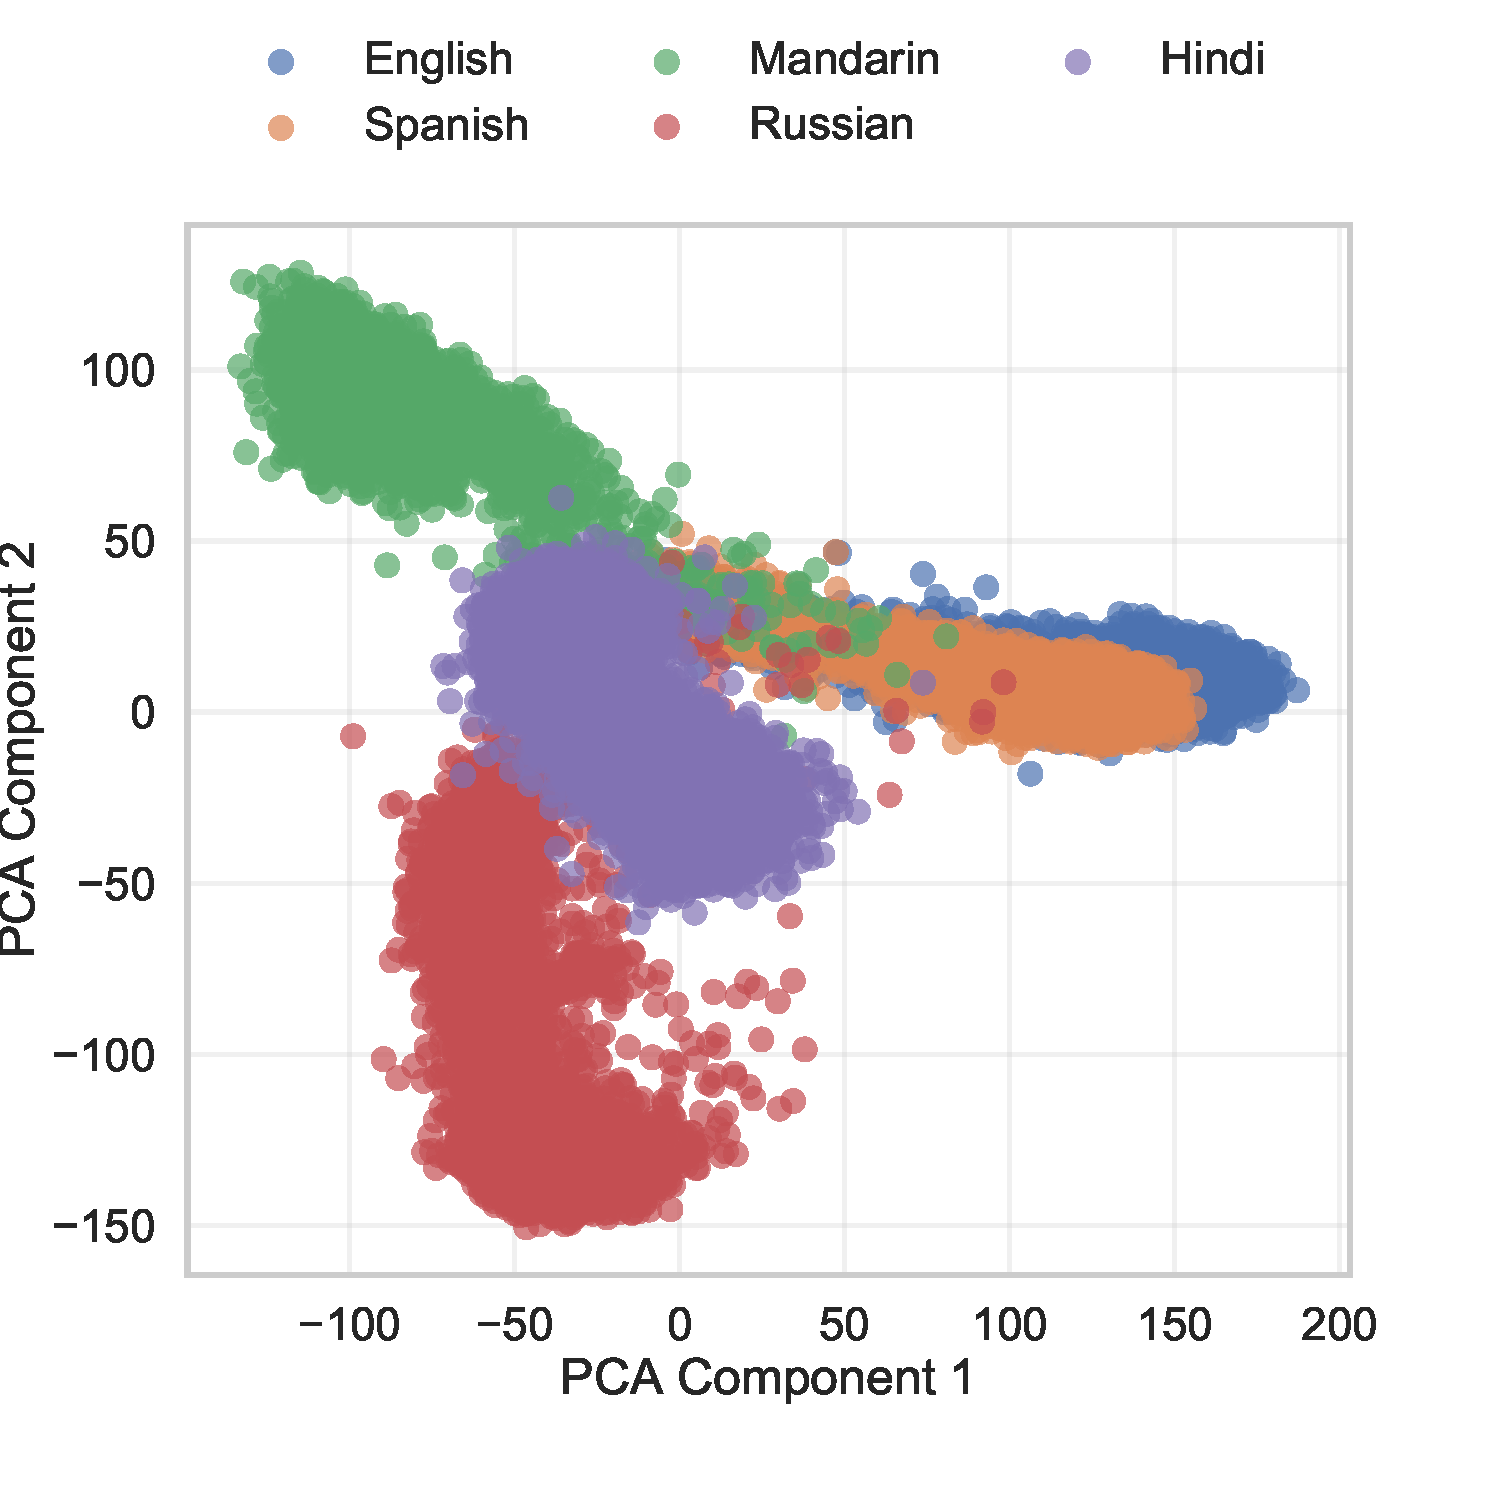
\includegraphics[width=1\linewidth]{images/language_map/multi/qwen/layer_28.pdf}
    \caption{Qwen}
    \label{fig:qwen_lang_map}
  \end{subfigure}
  \hfill
  \begin{subfigure}[b]{0.48\linewidth}
    \centering
    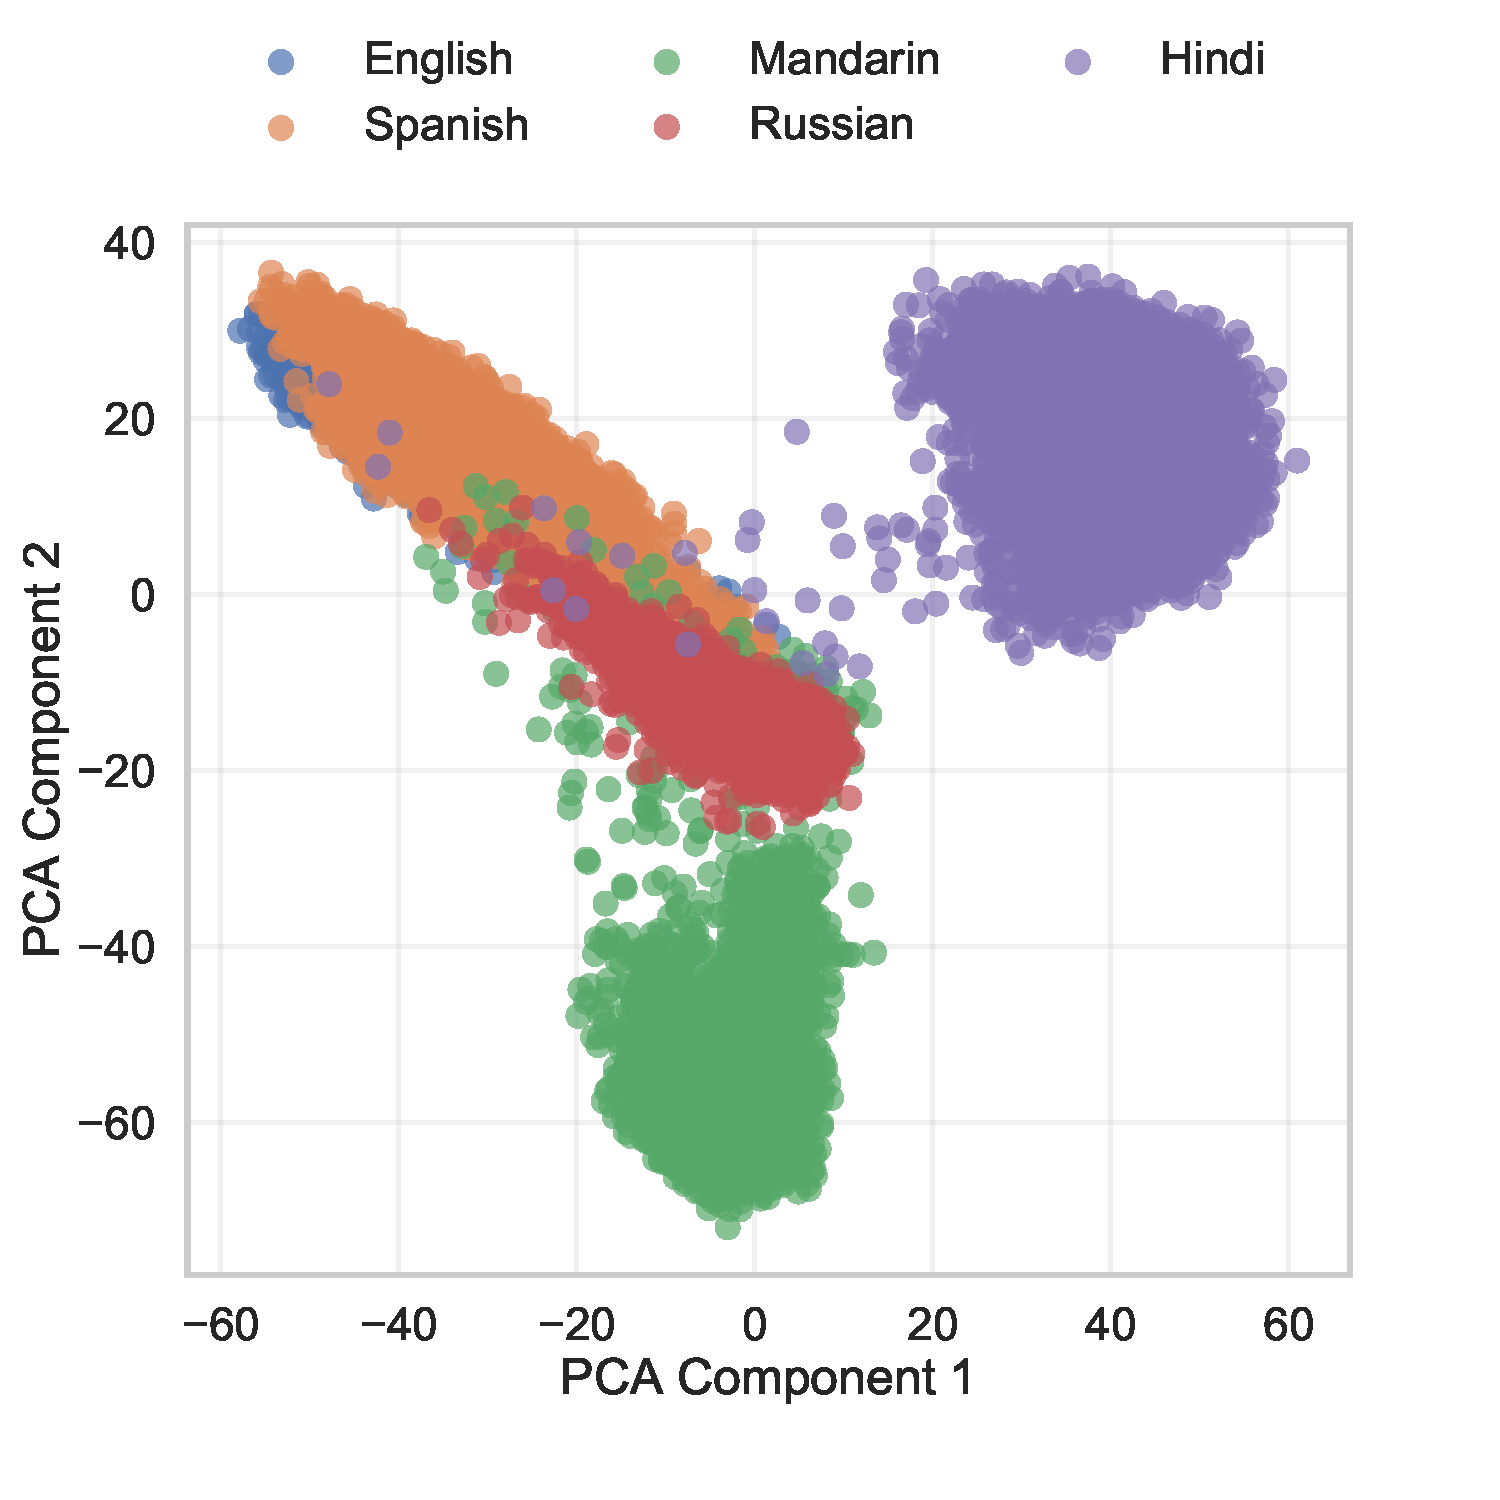
\includegraphics[width=1\linewidth]{images/language_map/multi/llama/layer_16.pdf}
    \caption{Llama}
    \label{fig:llama_lang_map}
  \end{subfigure}
  \caption{Final layer language map}
\end{figure*}

\begin{figure*}[ht]
  \centering
  \begin{subfigure}[t]{0.24\linewidth}
    \centering
    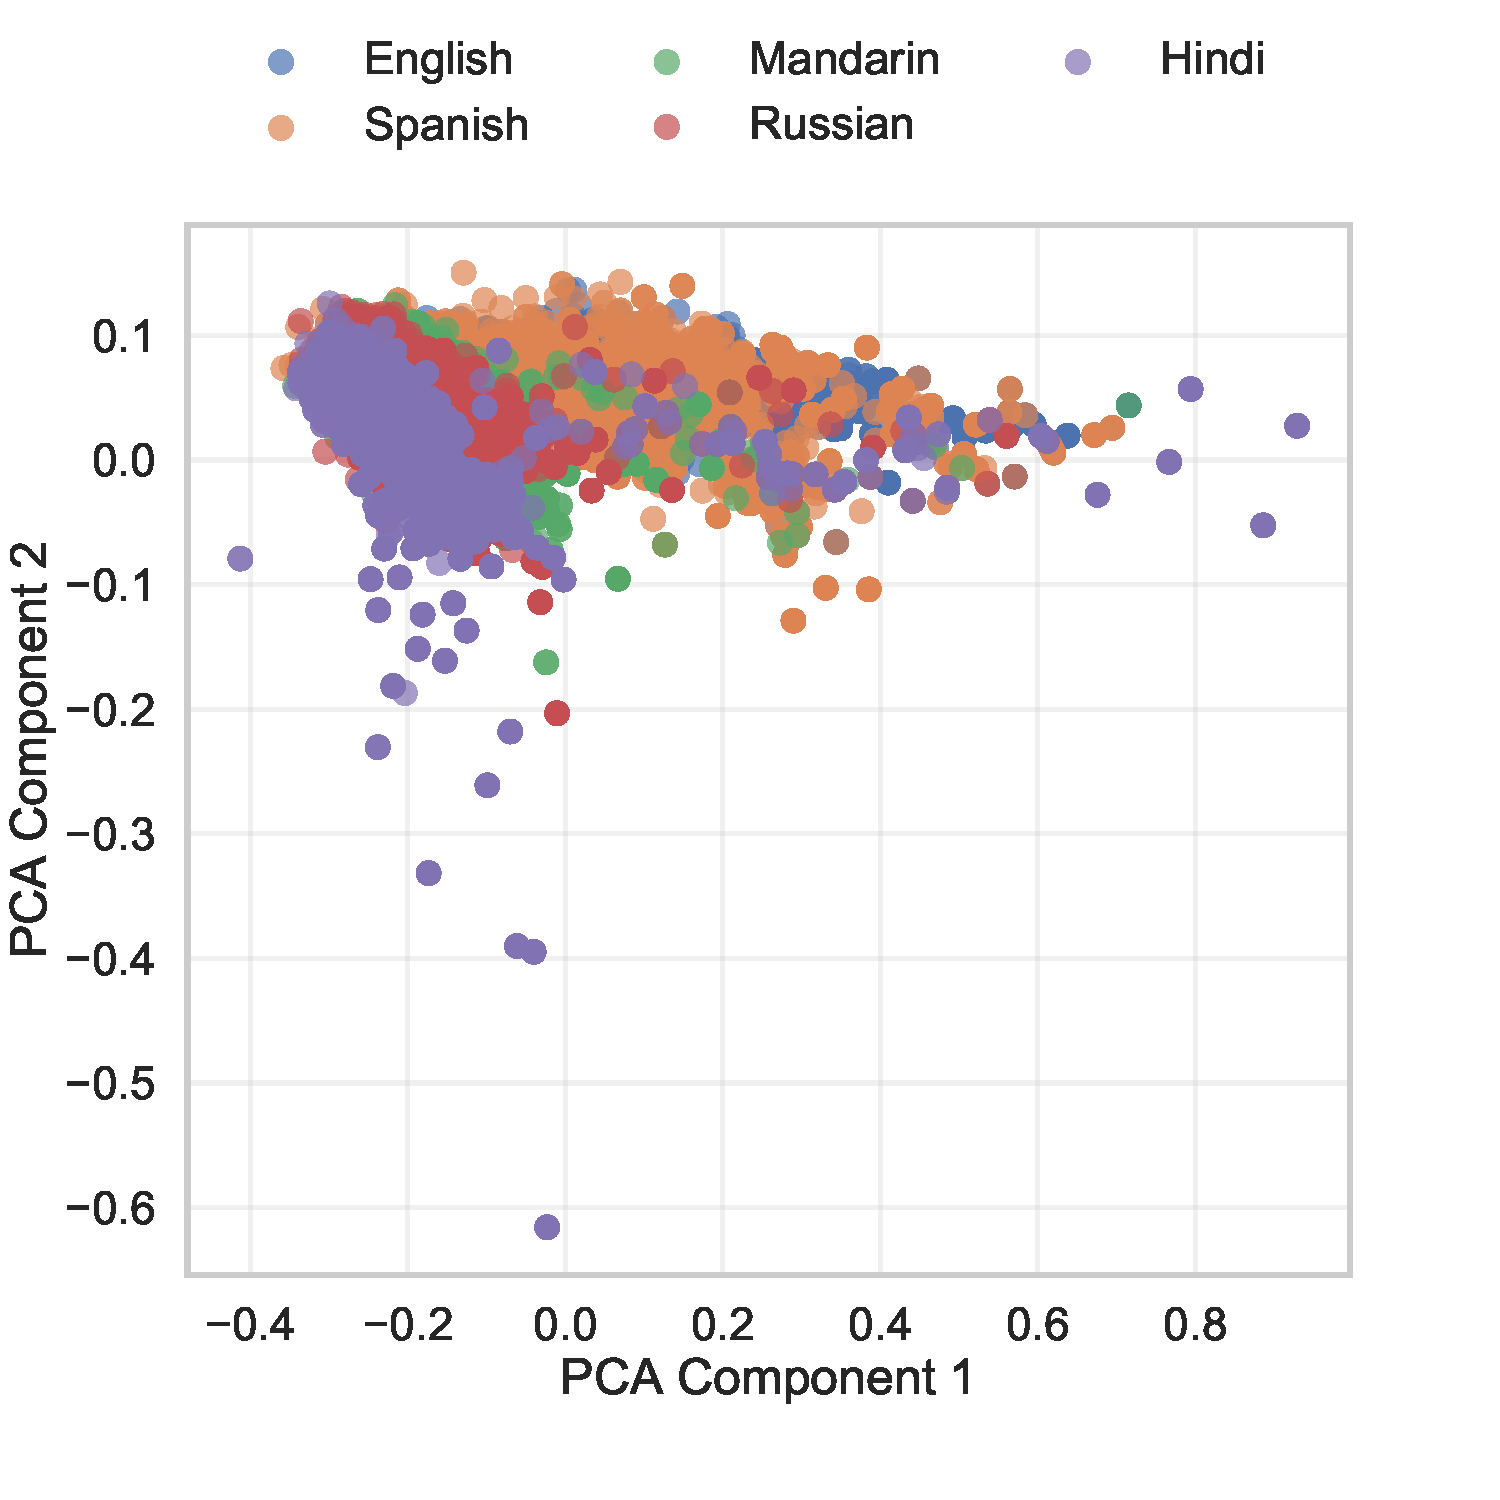
\includegraphics[width=1\linewidth]{images/language_map/multi/llama/layer_0.pdf}
    \caption{First layer}
    \label{fig:llama_lang_map_first}
  \end{subfigure}
  \hfill
  \begin{subfigure}[t]{0.24\linewidth}
    \centering
    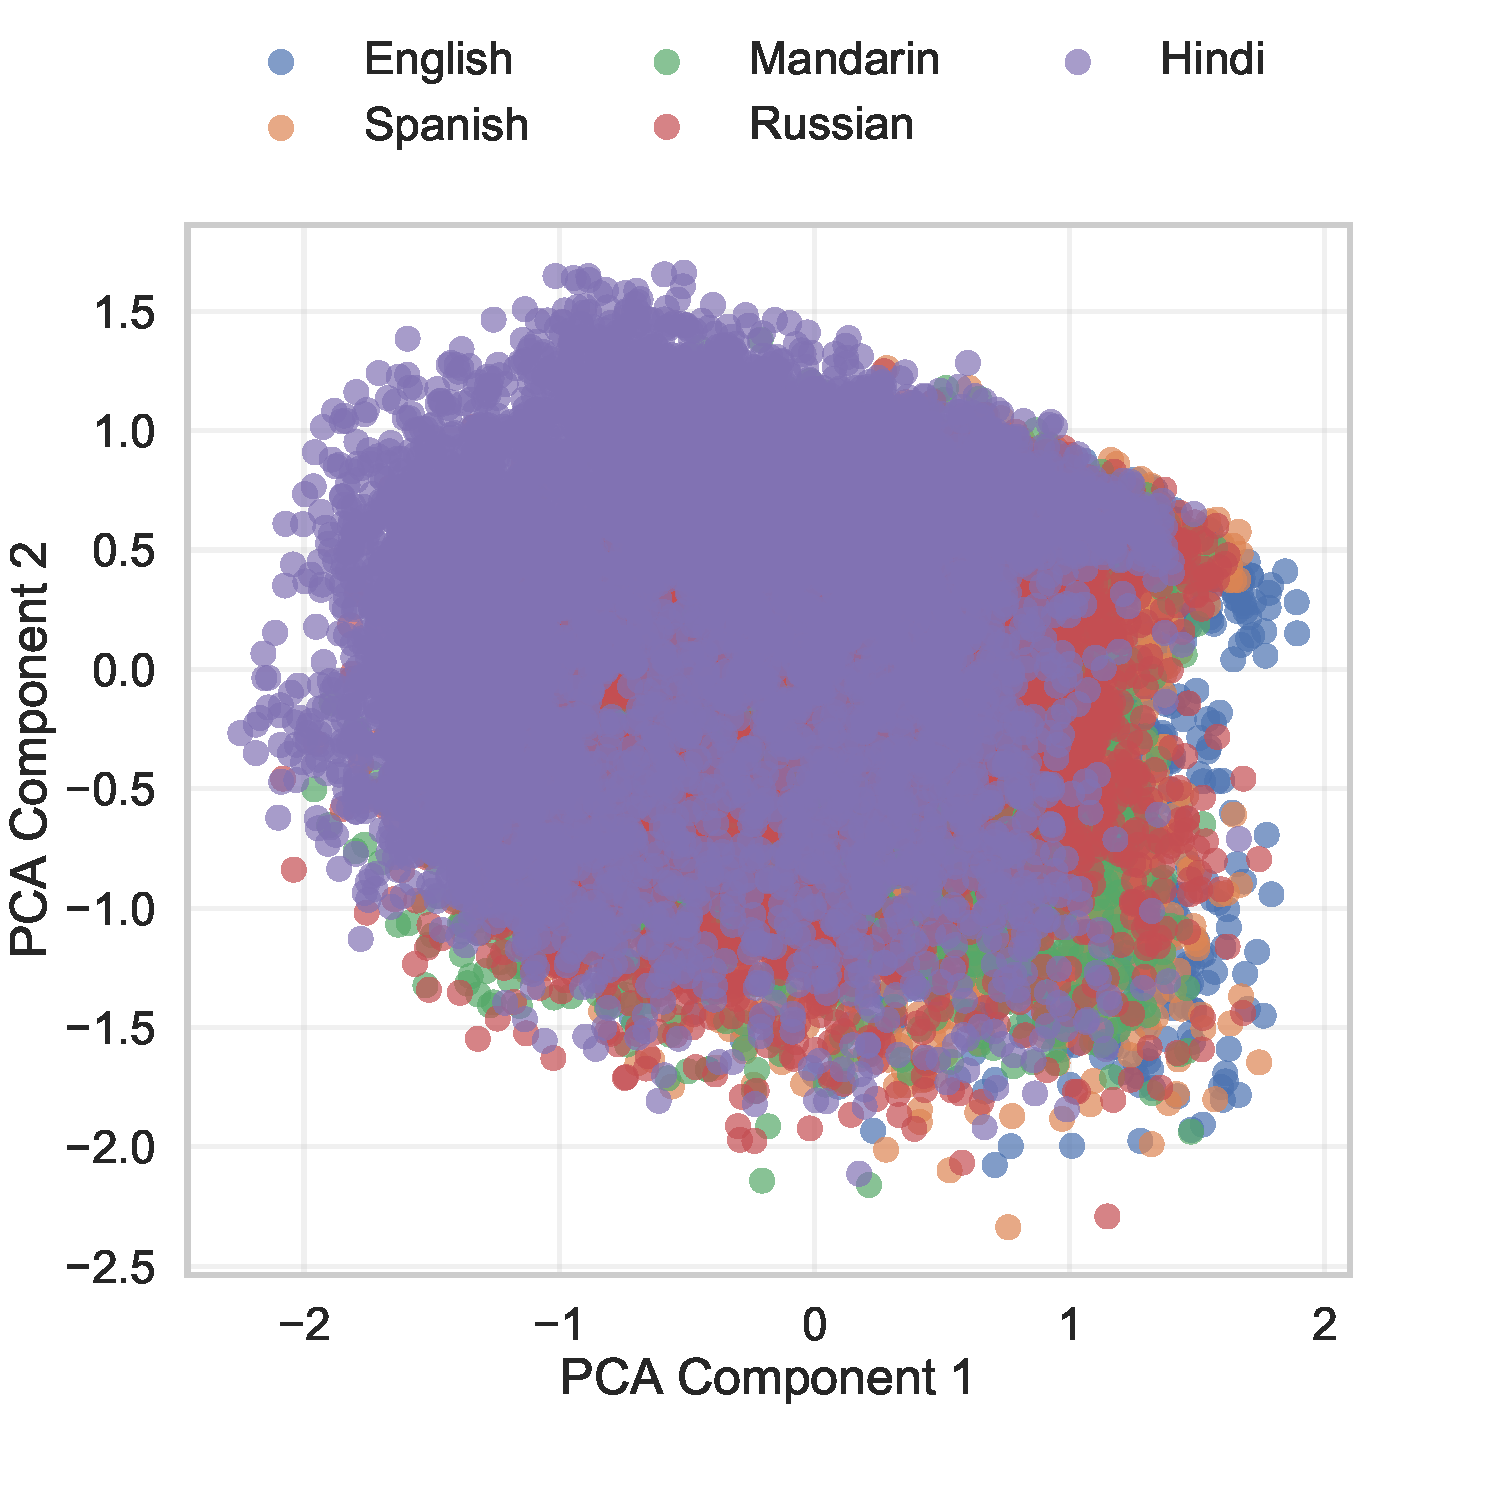
\includegraphics[width=1\linewidth]{images/language_map/multi/llama/layer_7.pdf}
    \caption{Mid layer}
    \label{fig:llama_lang_map_mid}
  \end{subfigure}
  \hfill
  \begin{subfigure}[t]{0.48\linewidth}
    \centering
    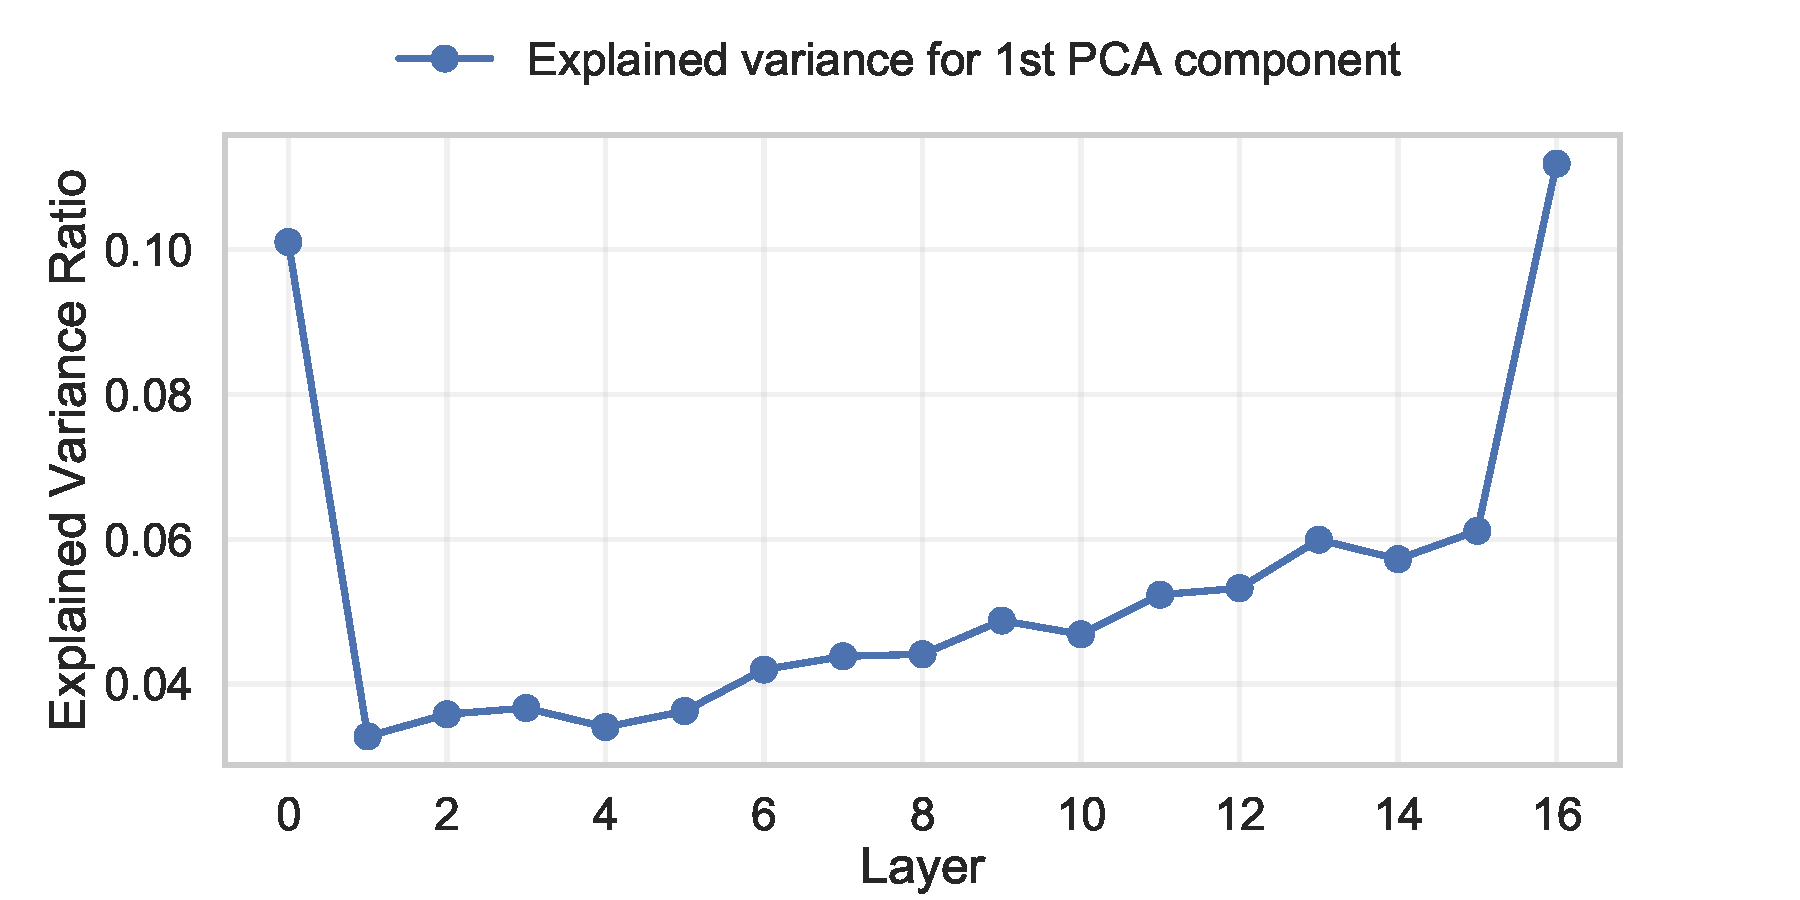
\includegraphics[width=1\linewidth]{images/language_map/multi/llama/explained_variance.pdf}
    \caption{Explained variance}
    \label{fig:llama_explained_variance}
  \end{subfigure}
  \caption{Llama layer-wise language maps and explained variance}
\end{figure*}

\begin{figure*}[ht]
  \centering
  \begin{subfigure}[t]{0.24\linewidth}
    \centering
    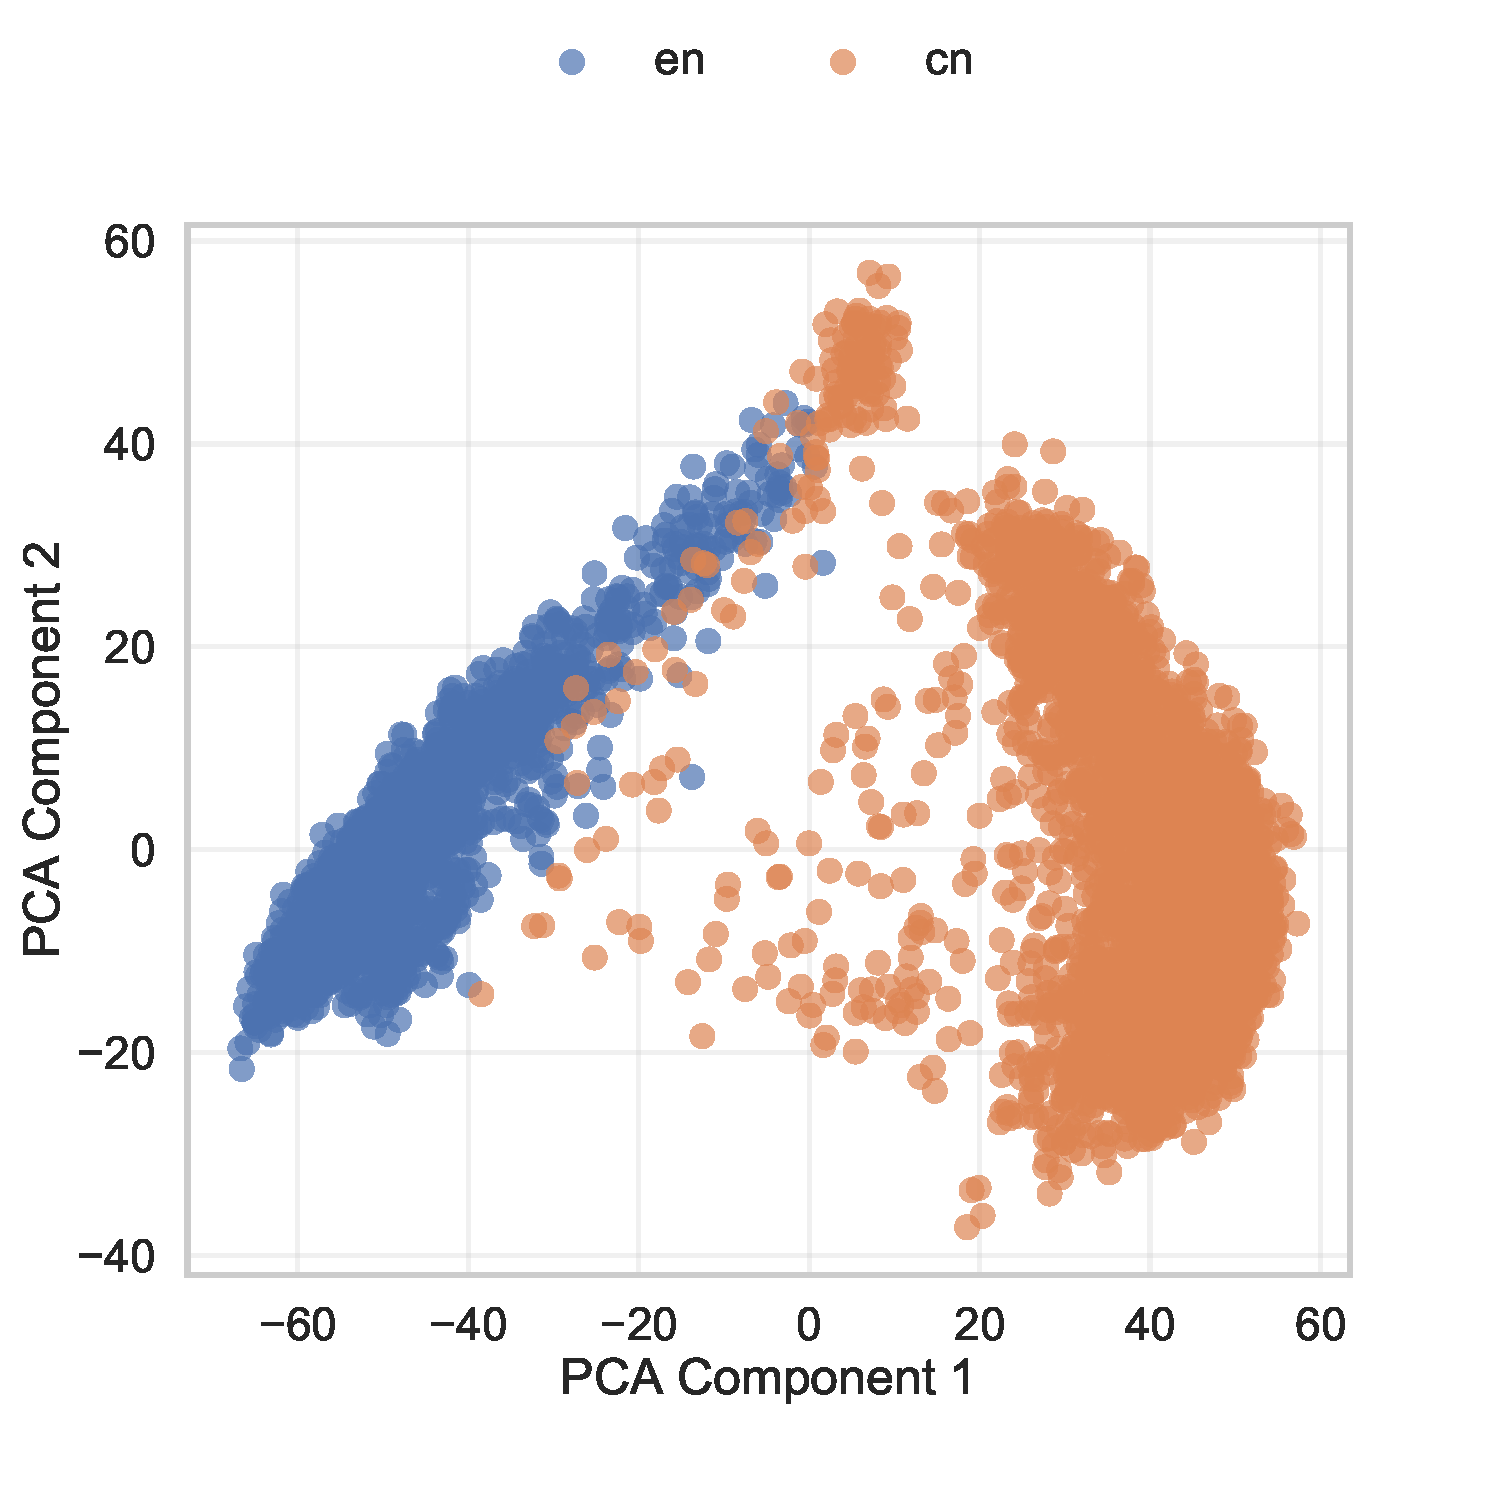
\includegraphics[width=1\linewidth]{images/language_map/en_cn/llama/layer_16.pdf}
    \caption{English - Chinese}
    \label{fig:llama_lang_map_en_cn}
  \end{subfigure}
  \hfill
  \begin{subfigure}[t]{0.24\linewidth}
    \centering
    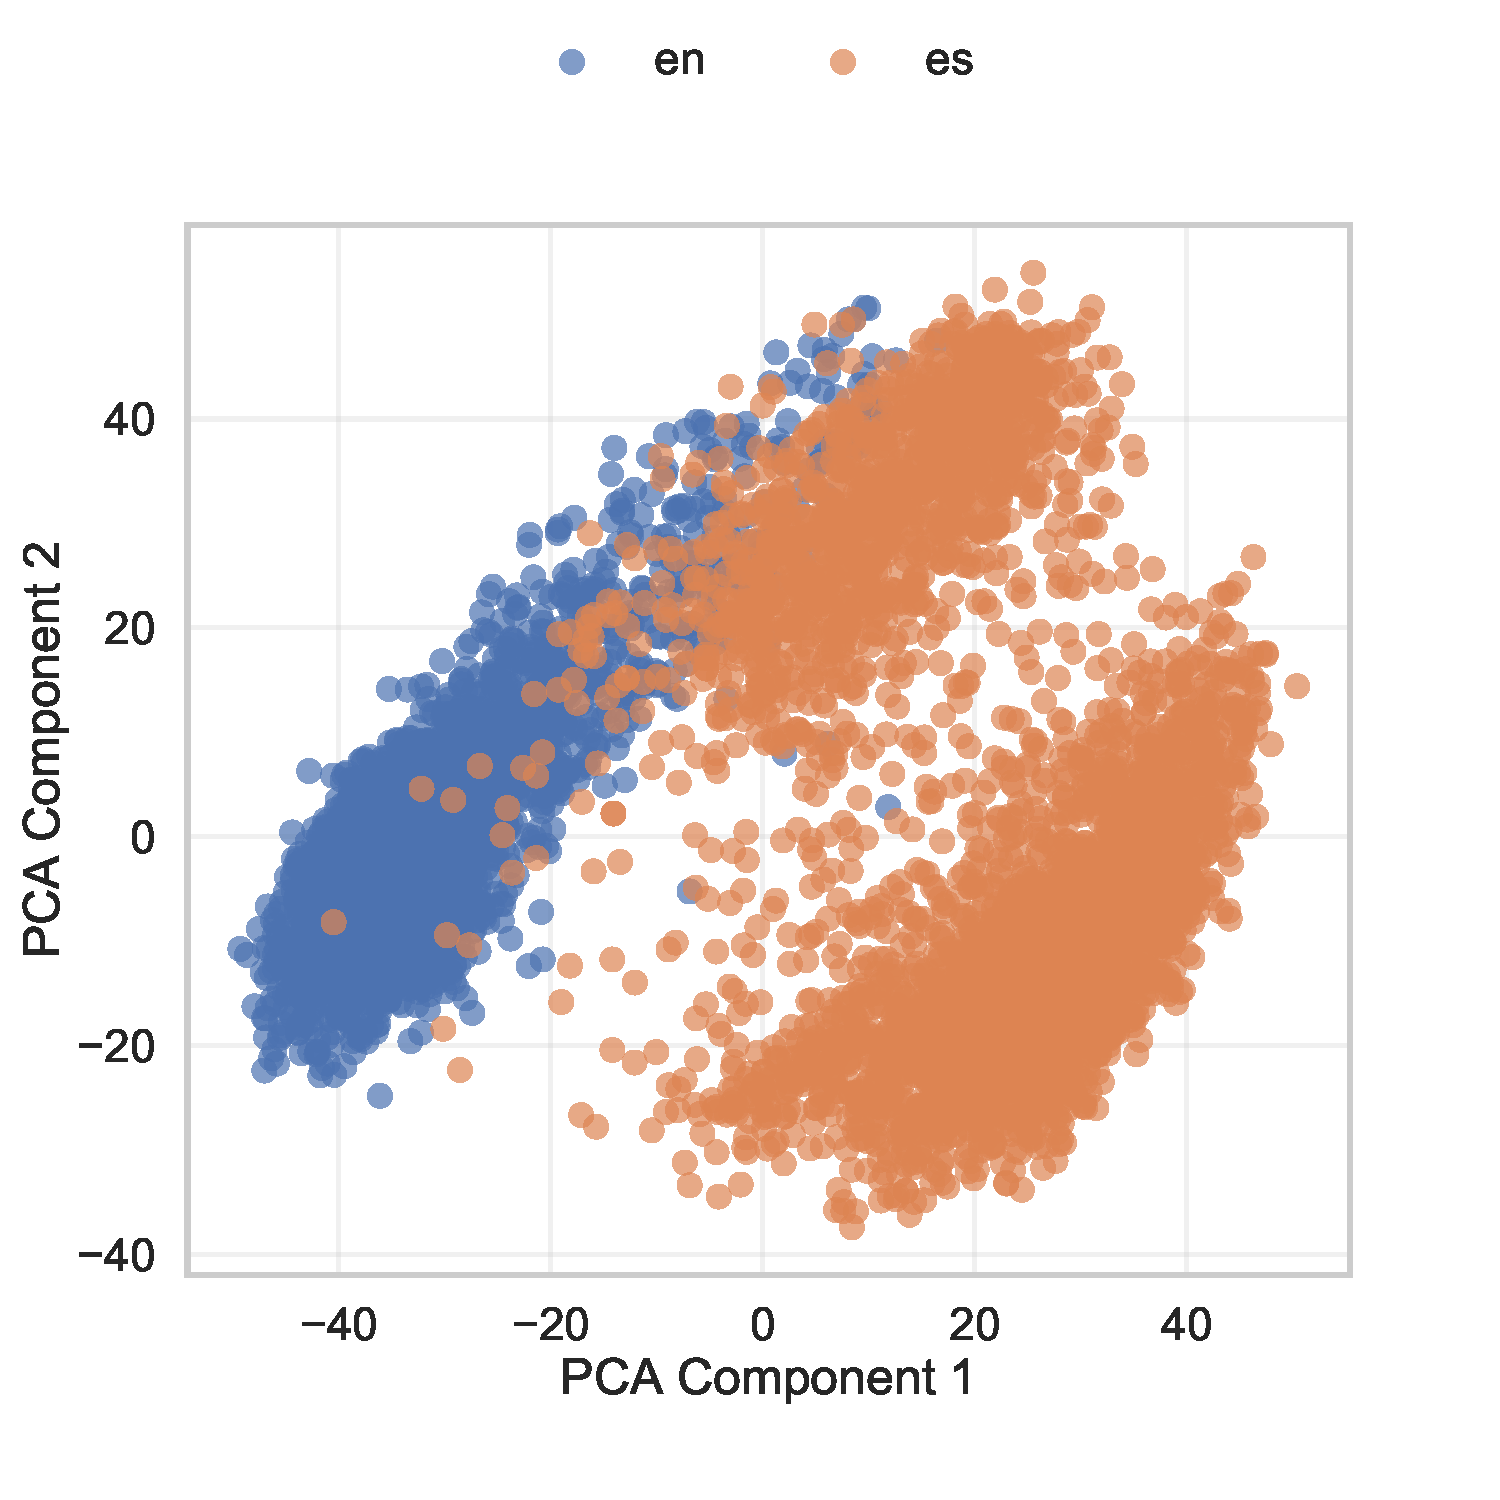
\includegraphics[width=1\linewidth]{images/language_map/en_es/llama/layer_16.pdf}
    \caption{English - Spanish}
    \label{fig:llama_lang_map_en_es}
  \end{subfigure}
  \hfill
  \begin{subfigure}[t]{0.24\linewidth}
    \centering
    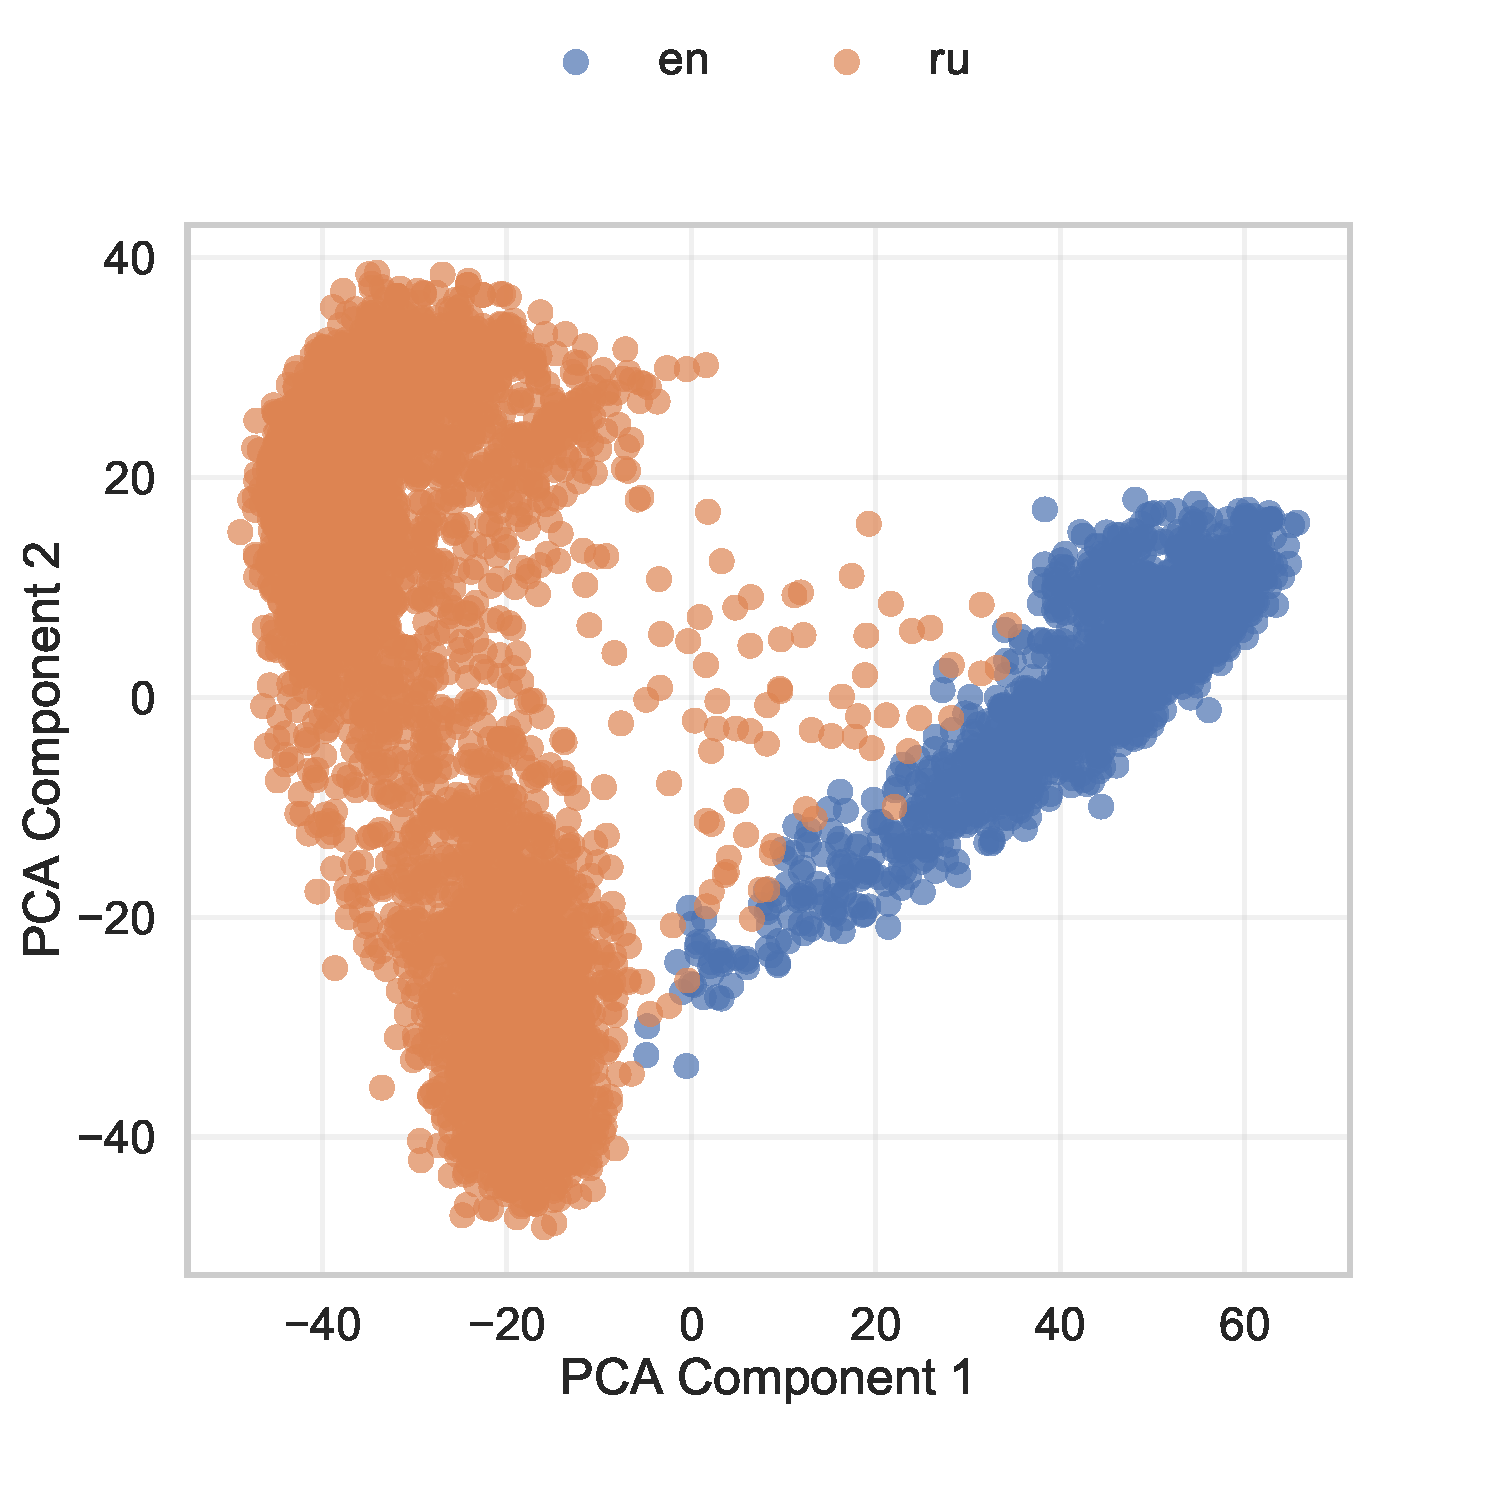
\includegraphics[width=1\linewidth]{images/language_map/en_ru/llama/layer_16.pdf}
    \caption{English - Russian}
    \label{fig:llama_lang_map_en_ru}
  \end{subfigure}
  \hfill
  \begin{subfigure}[t]{0.24\linewidth}
    \centering
    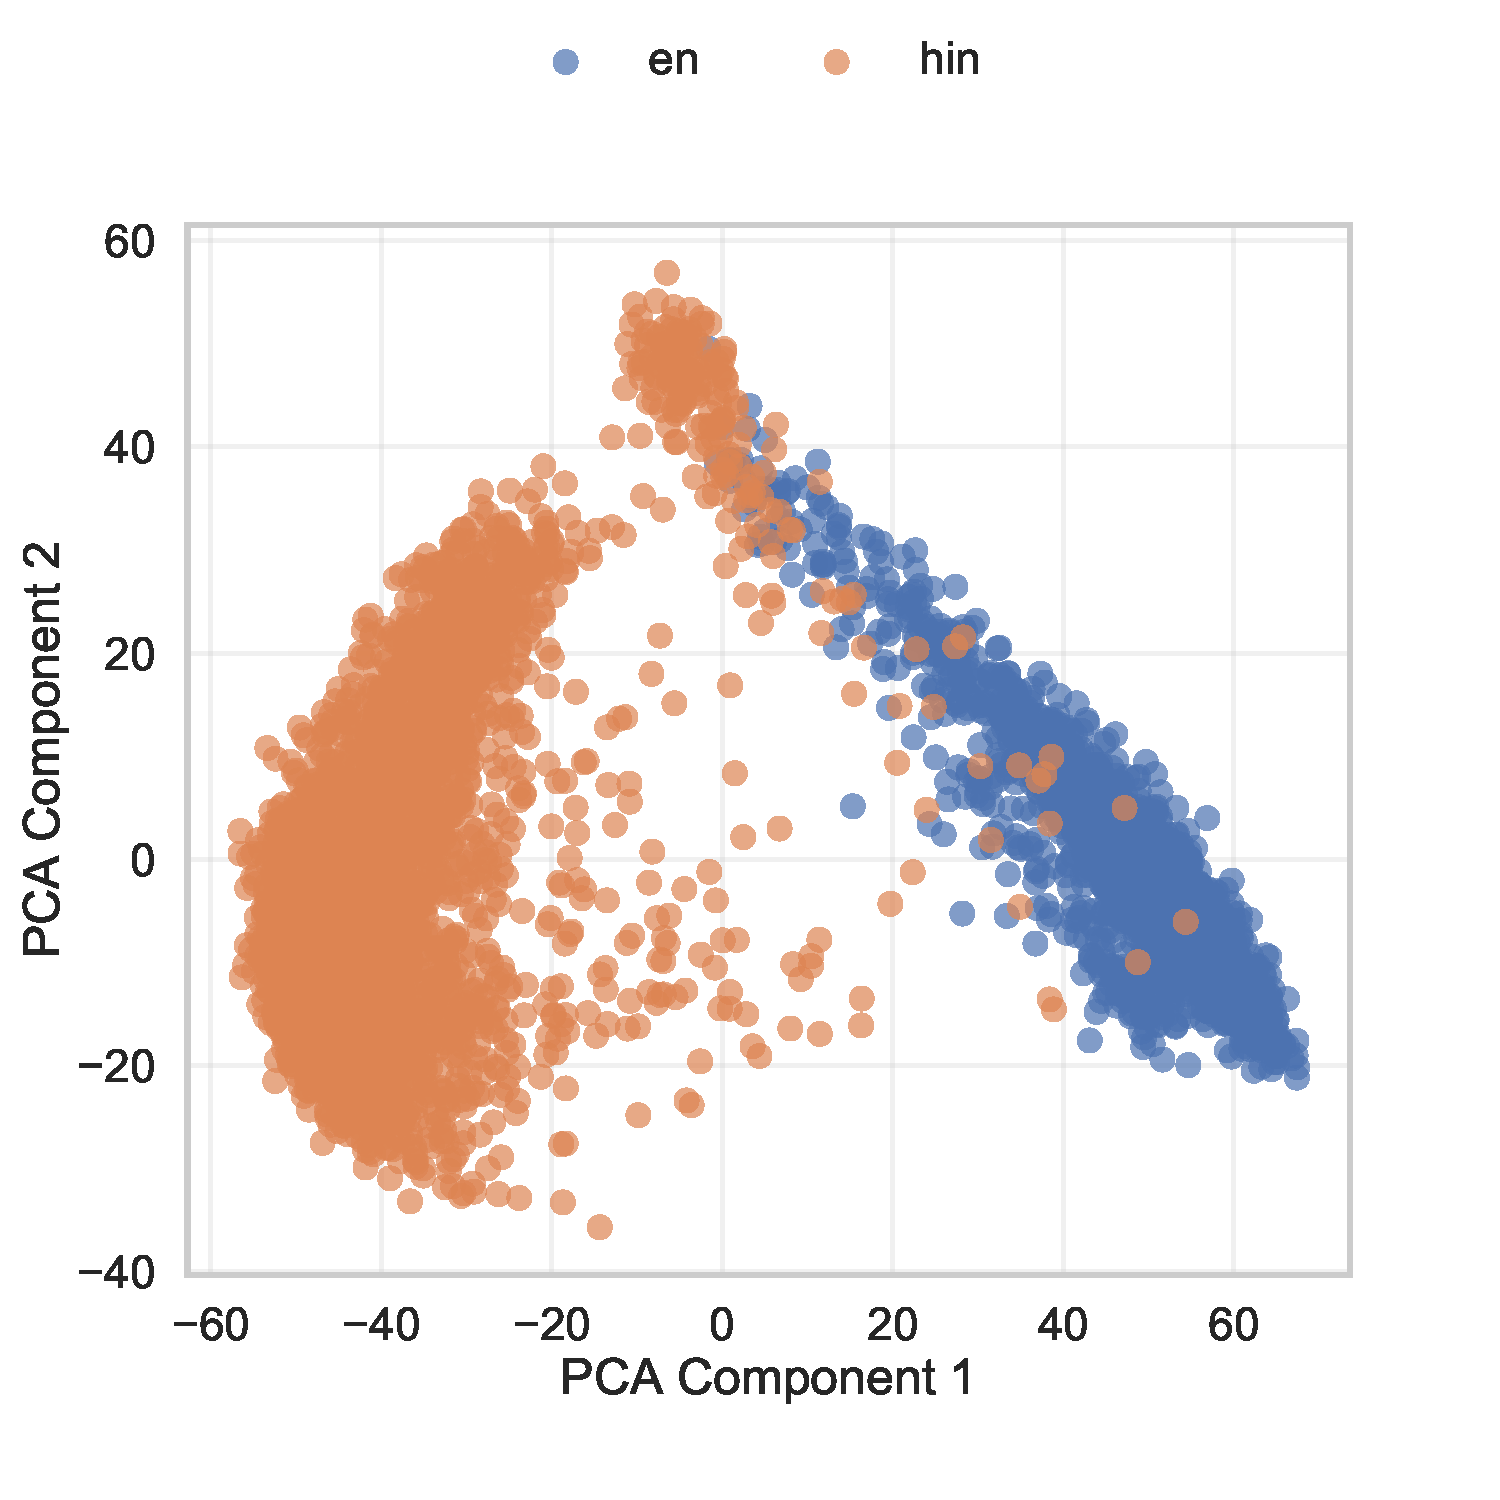
\includegraphics[width=1\linewidth]{images/language_map/en_hin/llama/layer_16.pdf}
    \caption{English - Hindi}
    \label{fig:llama_lang_map_en_hin}
  \end{subfigure}
  \caption{Llama final layer language maps for each language pair}
\end{figure*}

\subsection{Language direction identification}

\paragraph{Experimental setup.} Dataset: Flores Plus \cite{scaling-2024} with 50 parallel samples (English, Spanish, Russian, Chinese, Hindi) for PCA fitting and 100 for validation. Models: Qwen2.5-1.5B ~\cite{qwen2025qwen25technicalreport} and Llama-3.2-1B ~\cite{grattafiori2024llama3herdmodels}.

\paragraph{Language maps reveal emergent clustering.} Figure~\ref{fig:qwen_lang_map} and~\ref{fig:llama_lang_map} show final-layer embeddings projected onto the first two PCs.
Consistent with prior findings~\cite{conneau-etal-2020-emerging, wendler-etal-2024-llamas}, models organize identical content into tight, language-specific clusters with clear boundaries.
Languages within the Indo-European family (Spanish, Russian) cluster closer than typologically distant pairs (English--Chinese), suggesting PC1 captures coarse language distinction while PC2 encodes finer linguistic properties.

Figures ~\ref{fig:llama_lang_map_first} ~\ref{fig:llama_lang_map_mid} show layer-wise evolution:
clusters emerge loosely in early layers and sharpen dramatically in final layers.
Figure~\ref{fig:llama_explained_variance} reveals late-stage specialization for language identity.
Pairwise maps (Figures ~\ref{fig:llama_lang_map_en_cn}, ~\ref{fig:llama_lang_map_en_es}, ~\ref{fig:llama_lang_map_en_ru}, ~\ref{fig:llama_lang_map_en_hin}) confirm clean linear separability for all tested pairs.

\paragraph{Language prediction.} We train a logistic regression classifier on final-layer projections. Classifier trained only on the first principal component achieves near-perfect accuracy (0.96-1.00) across all language pairs and both models (Table~\ref{tab:clf}).
We observe decreased performance for the English-Spanish pair in both models, attributable to these languages being more closely related to each other.
\subsection{Language steering}

\paragraph{Next-token distribution evaluation.} We fit the steering module on Flores Plus with 200 parallel samples and test on 2,467 TED Talks \citep{banik2017tedtalks} samples with artificial code-switching.
Each sample is truncated to 20 words, split at the midpoint, and the second half is translated to the target language using Gemini 2.5 Flash via the OpenRouter API, producing texts that begin in English and switch mid-sentence.
Success is measured by comparing the next-token prediction distribution of the steered model against the English baseline via: KL divergence $\text{KL}(P_{\text{EN}} \| P_{\text{steered}})$, cosine similarity, and top-50 token overlap.

Table~\ref{tab:kl_cos_overlap} shows steering reduces KL divergence, increases cosine similarity and token overlap across all models and language pairs with a notable inefficiency on English-Hindi language pair.
The method shifts predictions from Spanish tokens (muy, bastante, tan) to their English equivalents (very, quite, so) while preserving semantic coherence (Table~\ref{tab:token_sample}).
We hypothesize that model-specific tokenization and training data balance play a key role. The Qwen model processed much more English and Chinese data, leading to more granular tokenization and better internal generalization for that pair.
At the same time, Hindi representation in the training corpus is usually much poorer.

\begin{table}[h]
  \centering
  \small
  \begin{tabular}{l l l}
    \hline
    Language pair & Qwen & Llama \\
    \hline
    English - Chinese & 10.15 / 0.02 / 3.69\% $\rightarrow$   & 9.05 / 0.05 / 4.47\% $\rightarrow$  \\
    & 4.52 / 0.22 / 26.46\% & 4.77 / 0.21 / 24.31\% \\
    English - Spanish & 7.25 / 0.12 / 11.41\% $\rightarrow$ & 6.52 / 0.12 / 11.45\% $\rightarrow$  \\
    & 4.90 / 0.18s / 20.23\% & 3.48 / 0.29 / 30.74\% \\
    English - Russian & 8.70 / 0.09 / 7.41\% $\rightarrow$  & 7.77 / 0.10 / 7.49\% $\rightarrow$  \\
    &5.40 / 0.23 / 25.45\% & 3.49 / 0.31 / 31.96\% \\
    English - Hindi & 9.60 / 0.04 / 11.23\% $\rightarrow$  & 8.06 / 0.06 / 6.54\% $\rightarrow$  \\
    &7.02 / 0.07 / 11.68\% & 6.13 / 0.16 / 25.88\% \\
    \hline
  \end{tabular}
  \caption{KL divergence / Cosine similarity / Top-50 token overlap (no steering $\rightarrow$ steering)}
  \label{tab:kl_cos_overlap}
\end{table}

\begin{table}[h]
  \centering
  \small
  \begin{tabular}{l c c c}
    \hline
    & & \multicolumn{2}{c}{Steered} \\
    \cmidrule(lr){3-4}
    Language pair & Unsteered & KL-opt. & CSI-opt. \\
    \hline
    English - Chinese  & 0.64 & 0.03 & 0.03 \\
    English - Spanish  & 0.62 & 0.23 & 0.11 \\
    English - Russian  & 0.59 & 0.02 & 0.01 \\
    English - Hindi    & 0.81 & 0.04 & 0.01 \\
    \hline
  \end{tabular}
  \caption{Code-Switching Index (CSI, $\downarrow$) of generated text (Llama-3.2-1B, $n=500$, code-switched input). English-only baseline: CSI~$= 0.02$. }
  \label{tab:gen_results}
\end{table}

\begin{table}
  \centering
  \small
  \begin{tabular}{l c c c}
    \hline
    & Qwen & \multicolumn{2}{c}{Llama} \\
    \cmidrule(lr){2-2} \cmidrule(lr){3-4}
    Language pair & KL-opt. & KL-opt. & CSI-opt. \\
    \hline
    English - Chinese & $-3.2$ & $-5.0$ & $-5.0$ \\
    English - Spanish & $-2.8$ & $-3.7$ & $-5.0$ \\
    English - Russian & $-2.2$ & $-3.5$ & $-4.0$ \\
    English - Hindi   & $+5.0$ & $-3.6$ & $-5.0$ \\
    \hline
  \end{tabular}
  \caption{Best steering strength coefficients. KL-optimized: from the distributional grid search; CSI-optimized: from the generation grid search.}
  \label{tab:steering_coeff}
\end{table}

\paragraph{Generation-based evaluation.} To complement the distributional analysis above, we evaluate steering on actual text generation using Llama-3.2-1B.
For each of 500 TED Talks samples per language pair, we generate 100-token continuations in three conditions: (A)~English-only input without steering, (B)~code-switched input without steering, and (C)~code-switched input with steering.
We measure code-switching in the generated output with the \emph{Code-Switching Index} (CSI)~\cite{gamback-das-2016-comparing} and a FastText classifier~\citep{joulin-etal-2017-bag}.

We evaluate two sets of steering coefficients (Table~\ref{tab:steering_coeff}).
Notably, the optimal steering coefficient (Table~\ref{tab:steering_coeff}) for Qwen English-Hindi is positive ($+5.0$), indicating the biggest variance comes not from the language component, but from some other component of unexplored nature.
Coefficients are highly fragile: small changes in magnitude can shift the model from fluent code-switched output to degenerate repetition.
Table~\ref{tab:qualitative} shows representative examples.

Table~\ref{tab:gen_results} shows that steering substantially reduces code-switching in generated text. CSI-optimized coefficients tend toward higher magnitudes, which improves language control but increases degeneration risk (see Limitations).


\section{Conclusion}

We introduced latent-space language steering, a lightweight inference-time method that mitigates unintended code-switching in multilingual LLMs without fine-tuning.
By extracting language directions via PCA on parallel translations, our approach enables precise control over language identity with negligible overhead - one dot product and vector subtraction per token.

Our empirical analysis across Qwen2.5 and Llama-3.2 models confirms that language identity concentrates in final layers with near-perfect linear separability.
This geometric structure enables both accurate language classification (95-99\% accuracy) and effective steering that reduces distributional divergence by up to 55\% and achieves 63--99\% Code-Switching Index reduction in generated text.

While distributional divergence is reduced by 40\% on average and generated text shows near-complete language conversion (TLC $> 0.77$ across all pairs), steering coefficients are highly fragile - aggressive values eliminate code-switching but can produce degenerate repetition, revealing a strong trade-off between language control and generation fluency.
Our approach offers a promising direction toward lightweight alternatives to fine-tuning for multilingual language control, though addressing the coefficient sensitivity remains important future work.


\section*{Limitations}

\begin{itemize}
  \item \textbf{Model scale and diversity.} Experiments limited to small models (1-1.5B parameters) and two architectures (Qwen2.5, Llama-3.2). Larger models and diverse architectures remain unexplored.

  \item \textbf{Incomplete reconstruction.} While the method achieves up to 55\% KL divergence reduction, the remaining gap indicates linear projections cannot fully reconstruct monolingual distributions, suggesting non-linear language-semantic interactions at the manifold level.

  \item \textbf{Dataset coverage.} Evaluation relies on Flores Plus and TED Talks (formal text). Conversational data, technical domains, and naturally occurring code-switching patterns are not tested. Our artificial code-switching setup produces mid-sentence switches at fixed positions, which may not reflect the morphosyntactic boundaries where natural code-switching typically occurs. Evaluation on naturalistic code-switching corpora such as the LinCE benchmark~\cite{aguilar-etal-2020-lince} is an important direction for future work.

  \item \textbf{Language typology.} Limited to Indo-European and Chinese languages. Low-resource languages, right-to-left scripts, and typologically distant languages (agglutinative, tonal) unexplored. Hindi showed the weakest improvement across both models, with KL reduction (24-27\%) but minimal gains in other distributional similarity metrics, suggesting tokenization or data balance issues.

  \item \textbf{Layer-wise steering.} Steering applied only to final layers based on empirical observation. Systematic exploration of multi-layer or adaptive steering strategies not conducted.

  \item \textbf{Evaluation metrics.} While we supplement distributional metrics (KL, JS divergence) with generation-based code-switching metrics (CSI, M-Index, I-Index), we do not evaluate semantic preservation or downstream task performance. Human evaluation of output quality remains needed.

  \item \textbf{Fluency--control trade-off and coefficient fragility.} Generation-based evaluation reveals that aggressive steering coefficients, while effective at eliminating code-switching (CSI~$< 0.01$ for English-Russian and English-Hindi), can produce repetitive or degenerate output patterns. Steering coefficients are highly fragile. Small changes in magnitude shift behavior from fluent code-switched text to degenerate repetition. The CSI-optimized coefficients cluster near the maximum tested values ($-5.0$), suggesting that direct optimization of generation metrics pushes toward an aggressive regime. Combining steering with constrained decoding or adaptive coefficient scheduling could mitigate this issue.

  \item \textbf{Steering calibration.} Optimal coefficients require manual grid search per language pair and depend on the optimization target (distributional vs.\ generation-based). Principled or adaptive selection methods not developed.

  \item \textbf{Efficiency benchmarking.} No rigorous latency profiling across hardware configurations or batch sizes to validate overhead claims for production deployment.

  \item \textbf{Bilingual, English-only steering.} Our evaluation steers exclusively toward English in bilingual settings. Multilingual steering and bidirectional steering are natural extensions that we leave to future work. The multilingual PCA maps (Figures~\ref{fig:qwen_lang_map},~\ref{fig:llama_lang_map}) suggest the geometric structure supports such extensions, as multiple language clusters are simultaneously separable.
\end{itemize}

\section*{Acknowledgements}

The research was supported by the Russian Science Foundation grant No. 25-11-00355, https://rscf.ru/project/25-11-00355/.


% Bibliography entries for the entire Anthology, followed by custom entries
\bibliography{custom}
\bibliographystyle{plainnat}

%\clearpage

%\appendix
%\section{Token overlap example}

\begin{table}[h]
  \small
  \centering
  \begin{tabular}{l l l}
    \hline
    Original & Unsteered & Steered \\
    \hline
    still & muy & very \\
    going & un  & surprised \\
    not & bastante & pretty \\
    so & tan & starting \\
    a & sor & working \\
    just & más & content \\
    really & a & rather \\
    in & empez & impressed \\
    very & de & quite \\
    sitting & content & -- \\
    quite & en & great \\
    pretty & enc & beginning \\
    here & aquí & answering \\
    thinking & pens & almost\\
    looking & realmente & fully \\
    kind & dese & \_\_\_\_ \\
    getting & completamente & \_\_ \\
    having & feliz & even \\
    actually & org & heart \\
    surprised & seguro & trying \\
    \hline
  \end{tabular}
  \caption{Top 20 token sample (Qwen, English-Spanish)}
  \label{tab:token_sample}
\end{table}

\section{Language classification results}

\begin{table}[h]
  \centering
  \begin{tabular}{l l l}
    \hline
    Language pair & Qwen & Llama \\
    \hline
    English - Chinese & 0.98 & 0.98 \\
    English - Spanish & 0.96 & 0.96 \\
    English - Russian & 0.99 & 0.99 \\
    English - Hindi & 0.98 & 1.00 \\
    \hline
  \end{tabular}
  \caption{Last layer language classifier accuracy}
  \label{tab:clf}
\end{table}

\section{Steering fragility example}

\begin{table}[ht]
  \centering
  \small
  \begin{tabular}{p{0.14\linewidth} p{0.80\linewidth}}
    \hline
    \multicolumn{2}{l}{\textbf{en-es:} \textit{``...I took on the task to ense\~{n}ar desarrollo global...''}} \\
    \hline
    Unsteered & \textit{de que un grupo de estudiantes suecos, que hab\'{i}an sido enviados a la Universidad de Harvard, me escribieron para pedir ayuda...} \\
    Steered & \textit{de that I had the opportunity to work with the first two editions of the course and I was very inspired by it...} \\
    \hline
    \multicolumn{2}{l}{\textbf{en-ru:} \textit{``...About 10 years ago, I took on the task to} [Russian text]\textit{...''}} \\
    \hline
    Degenerate steered & \textit{first year of the first year of the first year of the first year of the first year...} \\
    \hline
  \end{tabular}
  \caption{Generated continuations (Llama-3.2-1B, KL-optimized). Top: steering successfully redirects Spanish to coherent English. Bottom: steering eliminates Russian but produces degenerate repetition.}
  \label{tab:qualitative}
\end{table}

\end{document}